

We refer again to the system performance benchmarking analogy to describe the design considerations and methodology used in the proposed security benchmarking framework. In the performance benchmarking scenario, assume we are considering migrating from a corporate data center to the public cloud, and we want to estimate operating cost for multiple CSPs to base the comparison. Our strategy might begin by characterizing our data center's compute, network, and storage profiles and reproducing them on each of the candidate CSPs.  We can size the environments across CSPs by holding the workload parameters constant and tuning each cloud deployment until it  matches the expected baseline performance. Once we have established comparable deployment environments between clouds, we can then run the synthetic workload for the same duration on each provider and compare the costs incurred directly. After migration, benchmark tests can be scheduled to ensure SLAs are met and to inform system baseline heuristics and continuous monitoring systems. 

If we re-imagine this situation in terms of security metrics, the components needed for validation and verification begin to emerge. In this context, we are still comparing CSPs for cost efficiency, but the constraint is now to maintain the same security posture as our current system. 

The first step above was to establish the baseline performance metrics we intend to target on the systems under test. Obviously the target environments would be adjusted to account for differences in requirements - network latency and throughput might deviate based on proximity to the nearest cloud regional data center, or block storage capacity requirements might decrease given the availability of alternate cold storage services. 

Similarly, we can take a snapshot of the current security baseline by measuring any or all security metrics for the current state. This involves generating attack graphs and running simulations, or just interrogating the SIEM or other source of aggregated security telemetry for the current patch levels and AV signatures. After establishing the current baseline, we proceed with tuning the remote environments to match the baseline. This might involve scaling instance sizes to align with compute or network objectives, while tuning for security could lead to rewriting boundary service ACLs to meet the baseline attack surface target. When we tune the candidate environments to match the baseline, we are effectively calibrating our metrics for the current evaluation. After tuning is complete, running the synthetic workload (comprising network traffic generators, endpoint stressers, or disk/CPU/DB/etc relevant operation mixes for example) for a fixed amount of time should yield nearly the same results across all tuned metrics, with the exception being cost, which is the measurement we wanted to take.

\begin{figure}[ht]
\centering
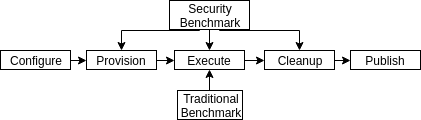
\includegraphics[width=.75\textwidth]{resource/img/ch_benchmarking/cloud_benchmarking_methodology.png}
\caption{Integrated Security Benchmarking Process}
\label{fig:benchmarking:boromir_arch}
\end{figure} 

To eliminate friction with evaluation and increase likelihood of adoption we have implemented our security benchmarks as an extension of the open source toolkit \textit{PerfKit Benchmarker}\cite{zaber_pkb}. PKB allows users to easily run benchmarks on various cloud providers without having to manually set up the infrastructure required for those benchmarks. PerfKit Benchmarker follows the 5 step process shown in Figure \ref{fig:benchmarking:boromir_arch} to automate each benchmark run. The Configuration phase processes command line flags, configuration files, and benchmark defaults to establish the final specification used for the run. The Provisioning phase creates the networks, subnets, firewalls and firewall rules, virtual machines, drives, and other cloud resources required to run the test. Benchmark binaries and dependencies like datasets are also loaded in this phase. The Execution phase is responsible for running the benchmarks themselves, and Teardown releases any resources created during the Provision phase. The Publishing phase packages the test results into a format suitable for further analysis such as  loading into a reporting system. The metadata returned from the Publishing phase can include verbose details about the actual infrastructure used during the test and timing information for each phase of the run along with the metrics returned from the benchmark itself, providing the level of detail needed to understand the benchmark results in context. 


% \begin{figure}[ht]
% \centering
% 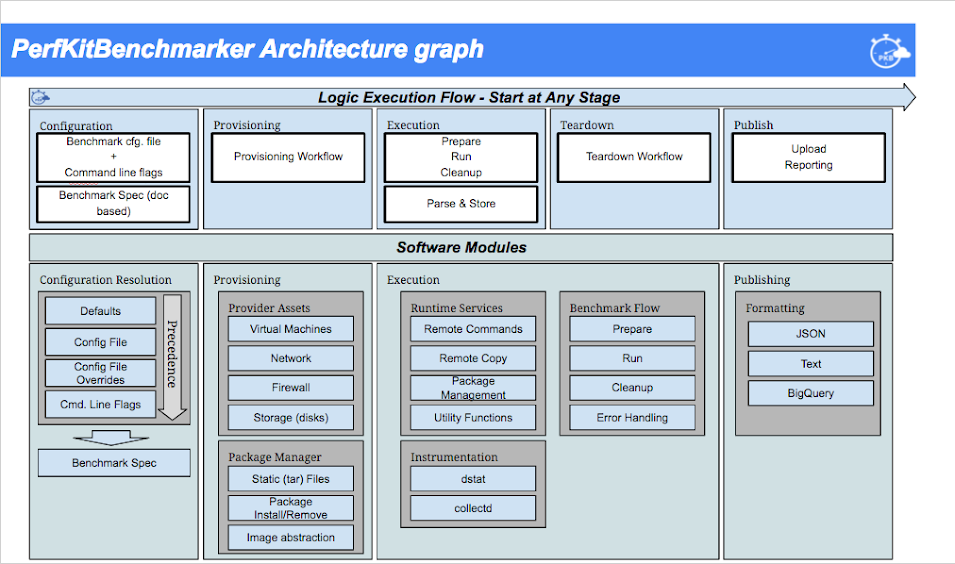
\includegraphics[width=.75\textwidth]{resource/img/ch_benchmarking/pkb_arch.png}
% \caption{Perfkit Benchmarker Run Stage Breakdown}
% \label{fig:benchmarking:pkb_arch}
% \end{figure} 
